%\documentclass{hotnets22}
% \documentclass[sigconf,10pt]{acmart}
\documentclass[letterpaper,twocolumn,10pt]{article}
\usepackage{usenix-2020-09}
\usepackage{amsmath}
\usepackage{amsthm}

\usepackage{xfrac}
\usepackage{algorithm}
\usepackage{algpseudocode}
\usepackage{times}  
\usepackage{hyperref}
% \usepackage{subfig}
\usepackage{tikz}
\usetikzlibrary{math}
\usepackage{pgfplots}
\usetikzlibrary{pgfplots.groupplots}
\usepackage{pgfplotstable}
\usepackage[subtle]{savetrees}
\usepackage[title]{appendix}

% axis style, ticks, etc
\pgfplotsset{every axis/.append style={
                    label style={font=\footnotesize},
                    tick label style={font=\footnotesize}  
                    }}

\usepackage{caption}
\usepackage{subcaption}
\usepackage{multirow}
\usepackage{tabularx}
\usepackage{array}
\usepackage{xspace}
\usepackage{soul}
\usepackage[normalem]{ulem}

\newcolumntype{s}{>{\hsize=.3\hsize\linewidth=\hsize}X}
\newcolumntype{D}{>{\hsize=.3\hsize\linewidth=\hsize}X}

\newcommand{\wdImg}{\dimexpr \linewidth-2\tabcolsep} %width of the image

\hypersetup{pdfstartview=FitH,pdfpagelayout=SinglePage}

\setlength\paperheight {11in}
\setlength\paperwidth {8.5in}
\setlength{\textwidth}{7in}
\setlength{\textheight}{9.25in}
\setlength{\oddsidemargin}{-.25in}
\setlength{\evensidemargin}{-.25in}

\newcommand{\rg}[1]{\textcolor{blue}{(\textbf{GR:} #1)}}
\newcommand{\vk}[1]{\textcolor{green}{(\textbf{VA:} #1)}}

\newtheorem{theorem}{Theorem}
\newtheorem{definition}{Definition}
\newtheorem{lemma}{Lemma}
\newtheorem{observation}{Observation}

% we have a big fig
\renewcommand{\floatpagefraction}{.8}%
% \renewcommand{\topfraction}{.8}
% \renewcommand{\bottomfraction}{.8}
\newcommand{\nftables}{\texttt{nftables}\xspace} 

% TODO: remove for the CR!
% \pagestyle{plain}
% \settopmatter{printfolios=true}

\begin{document}

% \conferenceinfo{HotNets 2022} {}
% \CopyrightYear{2022}
% \crdata{X}
% \date{}

%%%%%%%%%%%% THIS IS WHERE WE PUT IN THE TITLE AND AUTHORS %%%%%%%%%%%%

\title{Beyond Amdahl's Law: Achieving Superlinear Scaling with\\Distributed Self-adjusting Systems}

\author{Paper \#619, 12 + 7 pages}
% \author{Jonas Köppeler, Maciej Pacut, Tamás Lévai, Vamsi Addanki, Stefan Schmid, Gábor Rétvári}

\maketitle

\begin{abstract}
  Conventional wisdom suggests that linear scaling of the worker pool in a distributed system can result in at most a linear performance improvement. \sout{In this paper we show that distributed systems can be systematically architected to achieve  faster-than-linear (superlinear) scaling}. \hl{This paper introduces a design pattern for distributed systems that, in specific scenarios, achieves faster-than-linear (superlinear) scaling.} Our insight is that dispatching jobs to parallel workers so that the locality of reference in the workers' input increases, and implementing the workers with a self-adjusting algorithm to take advantage of the higher locality, jointly yield superlinear scaling. We demonstrate the potential use-cases for our design pattern in extensive simulations: scaling textbook self-adjusting algorithms we obtain 100--3,300x speedup using only 48 CPU cores, up to 70x beyond linear scaling. Then, we present two operational case studies. Using our optimization technique to scale a Memcached+PostgreSQL storage system we attain 2.3x faster than linear scaling. Then we re-engineer the Linux packet classifier to self-adjust with load, obtaining 800x speedup on synthetic traces and 220x speedup on real firewall traces with 32 CPU cores, resulting 5--25x times raw performance improvement compared to the vanilla Linux kernel.
\end{abstract}

% \tableofcontents

% a unique combination of \emph{locality-boosting load balancing} to spread load among workers implemented using \emph{self-adjusting data structures}.
  
\section{Introduction}\label{sec:introduction}


% use cases: multi-threaded app (RSS(HW) or RPS (SW)), cloud + cluster, job queues

% moore

% embarrassingly parallel

% amdahl limits

% superlinearity observed + perpeetum motion

% we show a systematic way to architect distributed systems to achieve SL scaling: LB-LB + SA

% sims + case study - results (360x in sims, 100x in benchmarks over Linux default)

% goals/nongoals

With the end of Moore's law, computing power in modern computing systems increasingly comes in the form of parallel processing resources.  A major obstacle faced by network engineers is how to harness this increasingly parallel computing power \cite{265065, 10.5555/3307441.3307467, 10.1145/2815400.2815423, 10.1145/3098822.3098826, 10.5555/3154630.3154639}.

In horizontally scaled applications, a load balancer dispatches jobs across a fleet of workers that process the jobs in parallel \cite{10.5555/3235491}, optionally synchronizing on shared state maintained in global storage.  In the context of \emph{web applications}, HTTP load balancers \cite{194966, 211279, 9552525} distribute requests across a swarm of backend web servers by hashing over the source IP address (``sticky sessions''). This way, requests from the same client will hit the same backend server, improving request locality and hence, performance. % Meanwhile, resource state is maintained in a key-value store or a relational database.
Multicore \emph{OS network stacks} \cite{211263, 10.1145/3359989.3365412, 10.1145/3452296.3472914} leverage the NIC to dispatch packets across the CPU cores. In order to avoid packet reordering and improve CPU cache performance, load balancing typically occurs by the NIC computing a hash over the packet header, e.g., the IP 5-tuple (RSS, RPS, etc.).  In massive-scale \emph{key-value stores} \cite{ghigoff2021bmc}, the key-space is hashed into multiple shards (partitions) and each shard is assigned to a separate server. Queries are distributed over the shards by hashing the requested key, and each shard processes only a portion of the key space.

The distributed system's overall goal is to achieve the greatest possible parallel speedup in terms of the the lowest time for executing a single task or the most tasks that can be finished during a given time period. Suppose a web app handles 100 requests per second using a single server. As we add another server, we expect a throughput of 200 requests per second. In reality, however, we usually obtain slightly less, and this is worsened as the system is scaled up further. This is because some fraction of most systems is inherently sequential and, therefore, bound to execute on a single CPU core. For instance, the web server replicas may need to synchronize write access to global state in a shared data store that cannot be scaled.  Beyond a certain threshold, parallel performance plateaus due to the sequential workload becoming a bottleneck.

The maximum speedup, measured as the ratio of the wall clock times of sequential and parallel execution, is formally described by Amdahl's law \cite{10.1145/1465482.1465560}. In general, the greater the serial portion $s$ compared to the parallelizable fraction of the code, the more performance is lost compared to an ``ideal'' linear scaling and the faster the system reaches saturation (see Fig.~\ref{fig:amdahl}). Amdahl's law is a cornerstone result in the parallel and high-performance computing practice and, despite often being debated \cite{10.1145/42411.42415}, extended \cite{4563876, 6280307,1580395,406581,6163449}, and misused \cite{10.5555/775339.775386}, it has remained one of the most useful tools in the system engineering toolbox \cite{10.5555/1951599}.

\begin{figure}[t]
  \centering
  % \includegraphics[width=0.8\linewidth]{fig/usl.png}
  \begin{small}
  \begin{small}
  \begin{tikzpicture}[remember picture]
    \begin{axis}[
      width=240pt,
      height=160pt,
      xlabel={\#threads},
      ylabel={Speedup},
      xlabel near ticks,
      ylabel near ticks,
      xmin=1,
      xmax=25,
      ymin=1,
      ymax=90,
      xtick={1,5,10,15,20,24},
      legend style = {
        anchor = north west,
        at = {(rel axis cs:0.01,0.98)},
        font=\scriptsize,
        % draw = none,
      },
      no markers
      ]
      % use TeX as calculator:
      \addplot[domain=1:25,black,densely dotted]{x};
      \addlegendentry{Linear scaling}

      \addplot[domain=1:25,black,densely dashed]{1/(0.01 + (1-0.01)/x)};
      \addlegendentry{Amdahl's law}

      \addplot[domain=1:25,black,solid]{1/(0.01 + (1-0.01)/x^2)};
      \addlegendentry{Superlinear scaling}

      \coordinate (insetPosition) at (rel axis cs:.98,0.23);
      % \addplot[domain=0:15,black,loosely dashed]{1/(0.4 + (1-0.4)/x)};
      % \addlegendentry{Amdahl's law ($\delta=0.4$)}

      % \addplot[domain=0:15,black,loosely dotted]{1/(0.4 + (1-0.4)/x^2)};
      % \addlegendentry{Proposed scaling law for MTF ($\delta=0.4$)}
    \end{axis}
    \begin{axis}[
      at={(insetPosition)},
      anchor={outer south east},
      width=105pt,
      height=85pt,
      tiny,
      % xlabel={\#cores},
      % ylabel={Speedup},
      xmin=1,
      xmax=450,
      ymin=0,
      ymax=110,
      % ytick={1,2,3,4,5},
      no markers]
      \addplot[domain=1:500,black,densely dotted]{x};
      \addplot[domain=1:500,black,densely dashed]{1/(0.01 + (1-0.01)/x)};
      \addplot[domain=1:500,black,solid]{1/(0.01 + (1-0.01)/x^2)};
    \end{axis}
  \end{tikzpicture}
\end{small}

%%% Local Variables:
%%% mode: latex
%%% TeX-master: "../distributed_mrf.tex"
%%% End:

\end{small}
  \caption{Linear scaling, Amdahl's law and the proposed scaling law ($s=0.01$). The inset shows the asymptotics.}
  \label{fig:amdahl}
\end{figure}

Inherent to Amdahl's law is that no system can scale faster than linear: doubling parallel resources will yield at most two times the performance. Curiously, there have been several genuine experimental reports of faster-than-linear (\emph{superlinear}) scaling exhibited by various distributed applications, including databases \cite{scalability-analyzed, 10.5555/1012889.1012894}, SDN analytics \cite{sdn-analytitcs}, high-performance computing \cite{556383, 7733347}, and multi-robot systems \cite{10.1007/978-3-319-77610-1}. In general, there seem to be two ways to ways to achieve superlinear scaling \cite{7733347, 80148}: do disproportionately less work in each worker as we scale the system \cite{7733347}, or add more resources per thread \cite{80148}. One typical example for the latter case is caching \cite{271208, 10.5555/1012889.1012894}: the more CPU cores the more (unshared) L1 cache space, which tends to make memory-bound\slash cache-bound applications disproportionately faster since the application now runs on a ``Bigger Machine'' \cite{80148} (see analysis in \S\ref{sec:background}).  Many authors, however, consider this phenomenon too elusive to be exploiting in engineering general distributed applications \cite{gunther-hotsos, 10.1145/2773212.2789974, 7733347, 80148}, or outright dismiss superlinear scaling all together \cite{gunther-hotsos}, concluding that ``superlinearity, although alluring, is as illusory as perpetual motion'' \cite{10.1145/2773212.2789974}.


In parallel computing, an embarrassingly parallel workload or problem (also called embarrassingly parallelizable, perfectly parallel, delightfully parallel or pleasingly parallel) is one where little or no effort is needed to separate the problem into a number of parallel tasks.[1] This is often the case where there is little or no dependency or need for communication between those parallel tasks, or for results between them.[2] 

goals:

\begin{itemize}
\item remove the misconception that linear scaling is the best one can achieve
\item general architecture
\end{itemize}


nongoals:

\begin{itemize}
\item present the fastest available packet classifier (but results speak forthemselves)
\end{itemize}

contributions:



%%% Local Variables:
%%% mode: latex
%%% TeX-master: "distributed_mrf"
%%% End:



\section{Background}\label{sec:background}

First we review Amdahl's scaling law and then we show a typical pattern to surpass it: distributed caching.

\subsection{Amdahl's Law}
\label{sec:amdahl-law}

A cornerstone result in parallel computing, Amdahl's law \cite{10.1145/1465482.1465560} establishes a firm limit on the performance gain one can obtain by distributing a computation task over multiple processors. Given a partially parallel program, denote the fraction of execution time spent % by a single-threaded execution
% by the processor 
in the serial part of the code by $s$, and the parallel fraction by $(1-s)$. Here, some code is ``serial'' if it cannot benefit from the improvement of the parallel computing resources, like single-threaded code, critical sections guarded by exclusion locks, etc. Denote by $T(k)$ the runtime (in seconds) of the program when executed on $k$ processors, and let $S(k)=\frac{T(1)}{T(k)}$ denote the performance improvement relative to a single-threaded execution (i.e., the \emph{speedup}). Then, the following relation holds (see Fig.~\ref{fig:amdahl}):
\begin{equation}\label{eq:amdahl}
S(k) = \frac{T(1)}{T(k)} = \frac{1}{s + \frac{1-s}{k}} \enspace .
\end{equation}

Here, the term $\frac{1-s}{k}$ establishes that the perfectly parallel part of the program executes $k$ times faster on $k$ processors than on a single core. By Amdahl's law, \emph{(i)} no code can scale faster than linear (i.e., $\frac{d S(k)}{d k} \le 1$, with equality exactly when $s=0$), \emph{(ii)} throwing additional workers on a computation task yields diminishing returns ($\frac{d S(k)}{d k}$ is decreasing in $k$) and \emph{(iii)} the asymptotics is limited by the serial part only ($\lim_{k\to \infty}S(k) = \frac1{s}$). 

% \subsection{Superlinear speedup}
% \label{sec:backgound-superlinear}

% The uniting idea of both parallel computing and multi-robot systems is that having multi-
% ple processors or robots working on a task decreases the processing time. Typically we desire
% a linear speedup, that is, doubling the number of processing units halves the execution time.
% Sometimes superlinear scalability is observed in parallel computing systems and more fre-
% quently in multi-robot and swarm systems. Superlinearity means each individual processing
% unit gets more efficient by increasing the system size—a desired and rather counterintuitive
% phenomenon.

% As superlinear speedups seem special, they were frequently discussed and studied [2, 3]. There
% even exists a proof showing the impossibility of superlinear speedups but it assumes fixed problem
% size [4]. Superlinear speedups are rather infrequently observed in parallel computing (e.g., cache-
% size effects [5]) compared to rather frequent observations in multi-robot and swarm systems (e.g.,
% inherently collaborative tasks [6]). When observed, superlinearity is often a discrete effect, such
% as a workpackage happening to fit into the processors cache [5] or a robot group being able to
% form a bucket brigade [7, 8]. Superlinear scalability has much potential that should be enough
% motivation to investigate it across different domains and to understand how one can provoke it.

% Many authors reported the existence of a superlinear
% speedup, but most of them only mentioned it as a side effect
% [4]. Besides reporting a superlinearity, other researchers briefly
% presented that the reason for achieving a superlinear speedup
% is because of the greater amount of cache memory in the
% parallel execution compared to the sequential [5].

\subsection{Distributed Caching}
\label{sec:backgound-dist-cache}

Critical to Amdahl's law is the assumption that the size of the individual sub-problems assigned to the workers remains constant as we scale the system (see also ``Gustafson's law'' \cite{10.1145/42411.42415}). Under this ``fixed size'' assumption \cite{556383}, faster-than-linear scaling is impossible \cite{10.1016/0167-8191(86)90024-4}. However, when this assumption fails, say, when the per-worker problem size gets progressively smaller or execution gets gradually faster as we add more parallel workers (``scaled size'' model \cite{556383}), superlinear\footnote{In this context, any function growing faster than $f(x) = x$ is considered ``superlinear'', despite that, for instance, $f(x) = 3x$ is still, mathematically speaking, linear. Some authors distinguish these functions using the term ``superunitary'' \cite{80148}. In line with the literature we will use the former terminology in the sequel.} scaling is often observed \cite{scalability-analyzed, sdn-analytitcs, 6483679, 10.1007/978-3-319-77610-1, dobb-1, dobb-2}. 

% there is an actual conclusion in `` SUPERLINEAR SPEEDUP IN HPC SYSTEMS: WHY AND WHEN?``: ``Mainly the superlinear speedup performance in persistent algorithms occurs due to the increased cache re- sources in the parallel computer architectures, the prefetching of shared variables in shared memory organization, or better scheduling in heterogeneous environments.''

% is can happen, for instance, due intricate interplays between per-worker problem size and available memory in certain specific applications, like distributed matrix multiplication and factorization \cite{6483679, 80148, 7733347}. In other cases superlinearity emerges out of pure luck, say because the code happens to progressively spend more time in faster subroutines as it is being scaled \cite{556383} or a parallel search algorithm finishes faster on some specific input \cite{80148}. And there are cases when superlinearity is observed due to simple benchmarking errors \cite{gunther-hotsos,10.1145/2773212.2789974}. But genuine superlinearity is most often observed in the context of 

The most prominent example for the scaled size model is \emph{distributed caching} \cite{scalability-analyzed, sdn-analytitcs, dobb-2} (for complete taxonomies see \cite{556383, 7733347, 80148}).  Most modern CPUs come with unshared Level-1 fast cache memory: the more CPU cores the more the cache memory the higher cache-hit rate at the workers and the faster the workers finish their sub-problems. This tends to speed up memory\slash cache-bound code disproportionately. Many distributed applications explicitly contain a fast-path\slash cache; e.g., \texttt{memcached} is often used as a fast cache for a ``slow'' web service \cite{180324,10.5555/1012889.1012894}, popular keys are cached in the OS kernel for fast key-value store access \cite{179747, ghigoff2021bmc}, FIB caches maintain the most recent IP routes to sidestep longest prefix matching \cite{rottenstreich2016optimal}, hierarchical flow caches serve as a fast-path in programmable software switches \cite{188960}, etc. All these workloads may benefit from the caches becoming more efficient as the system is scaled and, potentially, show superlinear speedup on certain workloads. % We stress, however, that faster-than-linear speedup is strictly contingent on the way work is distributed across workers so that subproblem sizes indeed reduce, otherwise cache efficiency remains constant and superlinear growth vanishes (see later).

\begin{figure}
  \centering
  \begin{small}
    \begin{small}
  \tikzmath
  {
    function lookup(\x)
    {
      if (\x < 10) then
      {
        return 0.1+0.9*(0.1*\x +(1-0.1*\x)*10)/\x;
      } else {
        return 0.1 + 0.9/\x;
      };
    };
    function dcache(\x)
    {
      return lookup(1.0)/lookup(\x);
    };
    function rrcache(\x)
    {
      return lookup(1.0)/(0.1+0.9*(0.1 +(1-0.1)*10)/\x);
    };
    function pcache(\x)
    {
      return lookup(1.0)/(0.1+0.9/\x);
    };
    \a = dcache(1);
    \b = lookup(1.0);
  }
  \begin{tikzpicture}
    \begin{axis}[
      width=250pt,
      height=170pt,
      xlabel={\#thread},
      ylabel={Speedup},
      xlabel near ticks,
      ylabel near ticks,
      xmin=0,
      xmax=20,
      ymin=0,
      ymax=67,
      xtick={1,5,10,15,20},
      legend style = {
        anchor = north west,
        at = {(0.01, 1.01)},
        font=\scriptsize,
        % draw = none,
      },
      % no markers
      ]
      \addplot[domain=0:25,black,solid]{dcache(x)};
      \addlegendentry{Hash-based load balancing}
      \addplot[domain=0:25,black,densely dotted]{rrcache(x)};
      \addlegendentry{Round robin load balancing}
      \addplot[domain=0:25,black,densely dashed]{pcache(x)};
      \addlegendentry{All requests hit the cache}
      % \node at (25,25) {\a, \b};
    \end{axis}
  \end{tikzpicture}
\end{small}

%%% Local Variables:
%%% mode: latex
%%% TeX-master: "../../hotnets22.tex"
%%% End:

\end{small}
\caption{Scaling laws for distributed caching: hash-based load balancing, lower envelope (round robin load balancing) and upper envelope (perfect cache hit rate with $k$ caches). Parameters: $s=0.1$, $\delta=0.1$ and $\rho=10$.}
  \label{fig:dcache-analysis}
\end{figure}

% refer to "Modeling Speedup (n) Greater than n" -> analysis

% assumption for the analysis? ``I think equation 2 should be explained much better. It is not at all obvious (not sure even correct) that hit rate scales linearly with threads (I think only true is delta << 1). What is $\rho$ exactly the ratio of (fetching time in the event of miss) / (fetching time in the event of a catch hit)?''

It is instructive to quantify superlinear speedup in this context using a simple model. Suppose a source emits uniformly distributed random requests for $m$ items and requests are distributed among $k$ workers, each using a separate fixed-size cache, by hashing on the request id.  Let the cache size be $c$. Initially, the cache hit rate for a single worker that processes all $m$ possible requests is $\frac{c}{m}=\delta$. Adding $k$ workers effectively partitions the requests into $k$ random buckets so that each worker will perceive uniformly distributed requests for only $\frac{m}{k}$ items, which improves the cache hit rate at each worker to $\frac{c}{\sfrac{m}{k}} = k\delta$ ($k\delta \le 1$). This puts the lookup time of the system of $k$ parallel caches to
\begin{align}\label{eq:dist-cache}
  T_c(k) = \begin{cases} s + \frac{1-s}{k}(k\delta + (1-k\delta)\rho) & \text{if } k\delta \le 1\\s + \frac{(1-s)}{k} & \text{otherwise}\end{cases} \enspace ,
\end{align}
where $\rho$ is the penalty for a cache miss event.

The speedup $S_c(k)=\frac{T_c(1)}{T_c(k)}$ is depicted in Fig.\ref{fig:dcache-analysis}. The lower envelope of the scaling profile is given by Amdahl's law for the system with random or round robin load-balancing. % ($\frac{T_c(1)}{s + \frac{1-s}{k}(\delta + (1-\delta)\rho)}$).
As $k$ grows the scaling profile progresses over a superlinear curve to an elevated Amdahl's law profile, representative of a system where \emph{all} $\frac{m}{k}$ requests are served by workers from fast memory.  % ($\frac{T_c(1)}{s + \frac{1-s}{k}}$).
Note that this occurs \emph{only} if request dispatching is chosen carefully to partition the item space. For instance, modulo hashing achieves this but a random or a round robin load balancer does not. This is because a round robin may send any item to any worker, which defeats the purpose of improving request locality at the workers' input. % and destroys superlinear scaling all together. % (see empirical evidence in the next Section).

Currently the only general methodology to achieve faster-than-linear scaling seems to be distributed caching, i.e., adding more fast memory to a system. Moving an application to a ``bigger machine'' \cite{dobb-2}, however, is not always feasible due to, e.g., physical or financial constraints.  In some cases caching cannot be used at all (e.g., for inherently stateful computations or complex database queries) or it introduces more overhead than it saves (e.g., for predominantly uniform input or rapidly changing data).  Moreover, caching comes with certain extra complexity \cite{271208} and often the required cache invalidation and eviction policies and data consistency mechanisms are too costly to implement in a massively distributed setting. Apart from caching, however, currently the only way to achieve faster-than-linear scaling is to rely on piecemeal problem-specific techniques, comprehensive domain knowledge, and pure luck. And even then, some compellingly argue that superlinear growth itself is a performance illusion, which goes against the very laws of nature much like perpetual motion \cite{gunther-hotsos, 10.1145/2773212.2789974}

% there is an actual conclusion in `` SUPERLINEAR SPEEDUP IN HPC SYSTEMS: WHY AND WHEN?``: ``Mainly the superlinear speedup performance in persistent algorithms occurs due to the increased cache re- sources in the parallel computer architectures, the prefetching of shared variables in shared memory organization, or better scheduling in heterogeneous environments.''

%%% Local Variables:
%%% mode: latex
%%% TeX-master: "distributed_mrf"
%%% End:



\section{Distributed Self-adjusting Systems}
\label{sec:architecture}

extend superlinear scaling beyond caching:
\begin{itemize}
\item when caches cannot be used due to, e.g., no locality, rapidly changing data, stateful computations, complex queries (classifier)
\item   due to complexity: cache invalidation, cache eviction, data consistency may be difficult to ensure in a distributed setting 
\end{itemize}

% One could convincingly argue that this is cheating, and a misuse of Amdahl's law \cite{10.5555/775339.775386}: by dropping additional cache instances to the system we effectively multiply the available fast memory, and this will trivially lead to faster access times. For multicore CPU systems this argumentation would clearly pass muster: since L2/L3 caches are typically shared across cores (but L1 caches are not!), so new threads will not improve performance, only worsen CPU cache contention \cite{manousis-sigcomm20, 211291}. We observe, however, that increasing the available fast memory is \emph{exactly the idea} in many common use cases, like adding \texttt{memcached} instances to a storage network or additional Redis replicas to sharded database cache.\footnote{Whether the superlinear scaling predicted by the model manifests itself with such real-life use cases is open for future research; we theoretize (without experimental evidence) that the answer is affirmative.}


\subsection{Self-adjusting algorithms}
\label{sec:sa-alg}

Temporal locality refers to the reuse of specific data and/or resources within a relatively small time duration. Spatial locality (also termed data locality[3]) refers to the use of data elements within relatively close storage locations.

In general, caches are just one example of the broader category of \emph{self-adjusting data structures}. A self-adjusting data structure can rearrange itself as queries are committed to it, in order to improve efficiency on future requests. In this context, a ``static cache'', which keeps an arbitrary set of items in fast memory without cache eviction, is not self-adjusting, while an LRU\slash LFU cache is. As another example, an AVL tree is not self-adjusting in that it can rearrange only with respect to the items \emph{stored} in it but not with respect to the queries \emph{committed} to it, whereas a splay tree is self-adjusting in that it can dynamically move popular items towards the root of tree, improving future access to the same or similar items \cite{SleatorT85Splay, BoseDL08, Avin0020}. Self-adjusting data structures are widely used in algorithms and computer systems, e.g., in computing point maxima and convex hulls~\cite{BentleyCL93}, organizing lists of identifiers in program compilation and interpretation~\cite{HesterH85}, detecting collisions in hash tables~\cite{HesterH85}, or compressing arbitrary input~\cite{BentleySTW86}. And indeed, every cache management scheme can be viewed as a self-adjusting data structure as well % , in that every algorithm for list reorganization gives rise to a different cache management algorithm~
\cite{SleatorT85}.  % Further self-adjusting data structures include splay trees~\cite{SleatorT85Splay}, self-adjusting skip lists~\cite{BoseDL08}, push-down trees~\cite{Avin0020}, or self-adjusting trees for storing geometric data \cite{ParkM12}.


\noindent%
\textbf{List lookup.} % MTF


Perhaps the best-known general self-adjusting data structure is the \emph{move-to-front list}. Suppose we wish to store a list of $m$ items in a way so that reordering, insertion and deletion is fast, while lookup is also ``reasonably'' efficient. A straightforward choice is a (singly) linked list. Here, the cost of accessing an item at position $i$ is exactly $i$. Then, a static linked list can easily be upgraded to a self-adjusting list using the move-to-front (MTF) heuristics: after accessing an item we move it to the front of the list (see Fig.~\ref{fig:mtf-example}). As such a reordering is supposed to be ``cheap'', MTF generally improves lookup time for future requests of the same item at minimal cost.


\begin{figure}
  \centering
  \includegraphics[width=.85\linewidth]{fig/mtf.pdf}
  \caption{A self-adjusting list containing nodes A,B,C and D serves the request to C and moves C to the front of the list to speed up future accesses to C.}
  \label{fig:mtf-example}
\end{figure}

Classic applications of MTF lists are information retrieval systems, compression~\cite{BentleySTW86}, etc. In network applications, however, where static linked lists enjoy wide applicability, e.g., for rule matching in OpenFlow and P4 reference software switches, packet classification in the Linux OS network stack (\texttt{iptables}), etc., so far we haven't seen many uses of the self-adjusting version, i.e., MTF lists. We imagine potential applications in packet classification (see later in \S\ref{sec:packet-classifier}), flow table lookup, evaluating rules in an intrusion detection system, etc.; in general, all networking use cases are relevant where ``matching'' a request against a list item is costly and the items do not lend themselves readily to be arranged into a fast lookup structure (like a search tree).



\noindent%
\textbf{Search trees.}


\begin{figure}
 \centering
 \begin{tikzpicture}[level distance=30pt,
   level 1/.style={sibling distance=30pt},
   level 2/.style={sibling distance=30pt},
   level 3/.style={sibling distance=30pt}]
   % Left
   \node[circle,draw,minimum size=0.5cm,inner sep=1pt] (3a) {3}
   child {node[circle,draw,minimum size=0.5cm,inner sep=1pt] (2a) {2}}
   child {node[circle,draw,minimum size=0.5cm,inner sep=1pt] (5a) {5}
     child {node[circle,draw,minimum size=0.5cm,inner sep=1pt] (4a) {4}}
     child {node[circle,draw,minimum size=0.5cm,inner sep=1pt] (6a) {6}}
   };
   % Right
   \node[circle,draw, minimum size=0.5cm, inner sep=1pt] (4b) at (5.5,0) {4}
   child {node[circle,draw,minimum size=0.5cm,inner sep=1pt] (3b) {3}
     child {node[circle,draw,minimum size=0.5cm,inner sep=1pt] (2b) {2}}
     child[missing] {}
   }
   child {node[circle,draw,minimum size=0.5cm,inner sep=1pt] (5b) {5}
     child[missing] {}
     child {node[circle,draw,minimum size=0.5cm,inner sep=1pt] (6b) {6}}
   };
   % Arrow
   \node (draw=none) at (2.8,-1.5) [font=\Large]{$\Rightarrow{Find(4)}$};
 \end{tikzpicture}
 \caption{Splay-tree with elements 2, 3, 4, 5, 6. After accessing node 4 it is moved to the root to speed up future accesses to it, while the search tree is kept almost perfectly balanced.}
 \label{fig:bst_root_3}
\end{figure}




\subsection{Locality-boosting load balancing}
\label{sec:lb-lb}

We call a request dispatching strategy that improves the temporal and\slash or spatial locality as experienced by the worker threads as a \emph{locality boosting load balancing policy}, and we identify such locality boosting load balancers as the first key ingredient in the superlinear scaling of distributed systems.

\begin{figure}
  \centering
  \includegraphics[width=.85\linewidth]{fig/schema.pdf}
  \caption{A locality boosting load balancer partitions the input sequence of a given locality into
    subsequences with higher locality. Self-adjusting data structures perform better on inputs with
    higher locality.}
  \label{fig:locality-boosting-lb}
\end{figure}

\subsection{Superlinear scaling}
\label{sec:arch-scaling}

% <PLACEHOLDER FOR MACIEK: discuss MTF lists without going into details, give examples with figs, and applications. Remember, we want to popularize the idea across the systems community, so be as gentle to practitioners as possible.>

show superlinear scaling with MTF

Indeed, a quick analysis proves that our MTF lists initially exhibit quadratic scaling over uniformly distributed requests. For a static linked list the worst-case lookup time is equals the length of the list, $m$, while for MTF it is rather the working set size $w\le m$ that determines lookup performance. This is because in MTF lists the working set will occupy the first $w$ positions in the list, which can be traversed in $w$ steps at most, and the inactive items will be moved to the back. Then, assuming that a hash-based load balancer partitions the $m$ possible requests over $k$ threads, each perceiving a working set size of $w=\frac{m}{k}$, the parallel MTF list will finish a lookup in amortized $\frac{m}{k}$ time. Plugging into Amdahl's law yields:
\begin{equation}\label{eq:mtf-perf}
  S_l(k) = \frac{T_l(1)}{T_l(k)} = \frac1{s + \frac{1-s}{k^2}} \enspace .
\end{equation}

For small values of $k$ we indeed obtain $O(k^2)$ scaling, despite that uniform request distribution is the worst case for self-adjustments. The fact that we see such speedups, even over a worst case input, hints at a great future potential over networking workloads that typically exhibit highly skewed request distributions~\cite{832484}.

\subsection{Simulations}
\label{sec:sims}

\begin{figure*}
  \begin{tabularx}{\textwidth}{D *{2}{s}}
    \hspace{28pt}% !TEX ROOT = ../distributed_mrf.tex
\pgfplotsset{
  RatePlot/.style = {
    tick pos = left,
    xtick align = outside,
    ytick align = outside,
    xlabel near ticks,
    ylabel near ticks,
    width=130pt,
    height=110pt,
    legend pos = north west,
    legend cell align = left,
    legend image post style = {scale = .9},
    legend style = {
      font = \scriptsize,
      inner sep = 0.5pt,
      row sep = -3pt,
    },
    legend image code/.code={  % make lines in legend images shorter
      \draw[mark repeat=2,mark phase=2, yshift=1pt]
      plot coordinates {
        (0cm,0cm)
        (0.15cm,0cm)    %% default is (0.3cm,0cm)
        (0.3cm,0cm)    %% default is (0.6cm,0cm)
      };%
    },
    mark size = 1pt,
    major tick length = 2,
    minor tick length = 1,
    label style = {font = \footnotesize},
    ylabel = {Throughput [Mpps]},
    xlabel = {number of CPU cores},
    xmin = 1, xmax = 32,
    ymin = 0,
  },
  SpeedupPlot/.style = {
    RatePlot,
    ylabel={Speedup},
  },
  ClassBenchGroupPlot/.style = {
    group/group size = 1 by 2,
    group/horizontal sep = 0pt,
    group/vertical sep = 10pt,
  },
  ClassBenchRatePlot/.style = {
    RatePlot,
    ylabel=,
  },
  ClassBenchSpeedupPlot/.style = {
    SpeedupPlot,
    ylabel=,
    xlabel=,
    xticklabels={},
  }
}

%%% Local Variables:
%%% mode: latex
%%% TeX-master: "../distributed_mrf.tex"
%%% End:

%
\begin{tikzpicture}
  \begin{axis}[%
    height=45pt,
    hide axis,
    xmin=10,
    xmax=50,
    ymin=0,
    ymax=0.4,
    legend style={
      draw=white!15!black,
      legend cell align=left,
      legend columns=2,
      font=\small}
    ]
    \addlegendimage{SelfAdjustingSimMark}
    \addlegendentry{Locality-boosting load balancer + Self-adjusting algorithm}
    \addlegendimage{StaticSimMark}
    \addlegendentry{Locality-boosting load balancer + Static algorithm}
    \addlegendimage{SelfAdjustingSimMark,mark=pentagon*}
    \addlegendentry{Roundrobin load balancer + Self-adjusting algorithm}
    \addlegendimage{StaticSimMark,mark=square}
    \addlegendentry{Roundrobin load balancer + Static algorithm}
  \end{axis}
\end{tikzpicture}

%%% Local Variables:
%%% mode: latex
%%% TeX-master: "../distributed_mrf"
%%% End:
\\
    \multirow{-11.9}{*}{\subcaptionbox{List lookup/uniform input\label{fig:multicore-list-uniform-100k}}{\pgfplotsset{
  RatePlot/.style = {
    tick pos = left,
    xtick align = outside,
    ytick align = outside,
    xlabel near ticks,
    ylabel near ticks,
    width=130pt,
    height=110pt,
    legend pos = north west,
    legend cell align = left,
    legend image post style = {scale = .9},
    legend style = {
      font = \scriptsize,
      inner sep = 0.5pt,
      row sep = -3pt,
    },
    legend image code/.code={  % make lines in legend images shorter
      \draw[mark repeat=2,mark phase=2, yshift=1pt]
      plot coordinates {
        (0cm,0cm)
        (0.15cm,0cm)    %% default is (0.3cm,0cm)
        (0.3cm,0cm)    %% default is (0.6cm,0cm)
      };%
    },
    mark size = 1pt,
    major tick length = 2,
    minor tick length = 1,
    label style = {font = \footnotesize},
    ylabel = {Throughput [Mpps]},
    xlabel = {number of CPU cores},
    xmin = 1, xmax = 32,
    ymin = 0,
  },
  SpeedupPlot/.style = {
    RatePlot,
    ylabel={Speedup},
  },
  ClassBenchGroupPlot/.style = {
    group/group size = 1 by 2,
    group/horizontal sep = 0pt,
    group/vertical sep = 10pt,
  },
  ClassBenchRatePlot/.style = {
    RatePlot,
    ylabel=,
  },
  ClassBenchSpeedupPlot/.style = {
    SpeedupPlot,
    ylabel=,
    xlabel=,
    xticklabels={},
  }
}

%%% Local Variables:
%%% mode: latex
%%% TeX-master: "../distributed_mrf.tex"
%%% End:

%
\begin{small}
  \begin{tikzpicture}
    \begin{axis}[
      width=165pt,
      height=142pt,
      xlabel={number of CPU cores},
      x label style={at={(0.5,0.04)}},
      ylabel={Speedup},
      % xlabel near ticks,
      % ylabel near ticks,
      y label style={at={(0.1,0.5)}},
      xmin=1,
      xmax=36,
      xtick={1,10,20,30},
      % xmax=48,
      % xtick={1,12,24,36,48},
      ymin=0,
      % ymax=170,
      legend style = {
        anchor = north west,
        at = {(0.01, 1.01)},
        font=\scriptsize,
        % draw = none,
      },
      % scaled y ticks=false
      % no markers
      ]
      % use TeX as calculator:
      \addplot[SelfAdjustingSimMark,mark size=2pt] table[x=thread,y=speedup] {fig/list/zipf-100k/multicore_mtf_modulo_zipf.txt};
      % \addlegendentry{Move-to-front/Local LB}
      \addplot[StaticSimMark,mark size=3pt] table[x=thread,y=speedup,each nth point={3}] {fig/list/zipf-100k/multicore_linkedlist_modulo_zipf.txt};
      % \addlegendentry{Linked-list/Local LB}
      \addplot[SelfAdjustingSimMark,mark=pentagon*,mark size=3pt] table[x=thread,y=speedup,each nth point={3}] {fig/list/zipf-100k/multicore_mtf_roundrobin_zipf.txt};
      % \addlegendentry{Move-to-front/Non-local LB}
      \addplot[StaticSimMark,mark=square,mark size=3pt] table[x=thread,y=speedup,each nth point={3}] {fig/list/zipf-100k/multicore_linkedlist_roundrobin_zipf.txt};
      % \addlegendentry{Linked list/Non-local LB}
    \end{axis}
  \end{tikzpicture}
\end{small}

%%% Local Variables:
%%% mode: latex
%%% TeX-master: "../../../distributed_mrf.tex"
%%% End:
}}%
    & \hspace{8pt}\subcaptionbox{List lookup/Zipf input\label{fig:3}}{\pgfplotsset{
  RatePlot/.style = {
    tick pos = left,
    xtick align = outside,
    ytick align = outside,
    xlabel near ticks,
    ylabel near ticks,
    width=130pt,
    height=110pt,
    legend pos = north west,
    legend cell align = left,
    legend image post style = {scale = .9},
    legend style = {
      font = \scriptsize,
      inner sep = 0.5pt,
      row sep = -3pt,
    },
    legend image code/.code={  % make lines in legend images shorter
      \draw[mark repeat=2,mark phase=2, yshift=1pt]
      plot coordinates {
        (0cm,0cm)
        (0.15cm,0cm)    %% default is (0.3cm,0cm)
        (0.3cm,0cm)    %% default is (0.6cm,0cm)
      };%
    },
    mark size = 1pt,
    major tick length = 2,
    minor tick length = 1,
    label style = {font = \footnotesize},
    ylabel = {Throughput [Mpps]},
    xlabel = {number of CPU cores},
    xmin = 1, xmax = 32,
    ymin = 0,
  },
  SpeedupPlot/.style = {
    RatePlot,
    ylabel={Speedup},
  },
  ClassBenchGroupPlot/.style = {
    group/group size = 1 by 2,
    group/horizontal sep = 0pt,
    group/vertical sep = 10pt,
  },
  ClassBenchRatePlot/.style = {
    RatePlot,
    ylabel=,
  },
  ClassBenchSpeedupPlot/.style = {
    SpeedupPlot,
    ylabel=,
    xlabel=,
    xticklabels={},
  }
}

%%% Local Variables:
%%% mode: latex
%%% TeX-master: "../distributed_mrf.tex"
%%% End:

%
\begin{small}
  \begin{tikzpicture}
    \begin{axis}[
      width=165pt,
      height=142pt,
      xlabel={number of CPU cores},
      x label style={at={(0.5,0.04)}},
      ylabel={Speedup},
      % xlabel near ticks,
      % ylabel near ticks,
      y label style={at={(0.1,0.5)}},
      xmin=1,
      xmax=36,
      xtick={1,10,20,30},
      % xmax=48,
      % xtick={1,12,24,36,48},
      ymin=0,
      % ymax=170,
      legend style = {
        anchor = north west,
        at = {(0.01, 1.01)},
        font=\scriptsize,
        % draw = none,
      },
      % scaled y ticks=false
      % no markers
      ]
      % use TeX as calculator:
      \addplot[SelfAdjustingSimMark,mark size=2pt] table[x=thread,y=speedup] {fig/list/zipf-100k/multicore_mtf_modulo_zipf.txt};
      % \addlegendentry{Move-to-front/Local LB}
      \addplot[StaticSimMark,mark size=3pt] table[x=thread,y=speedup,each nth point={3}] {fig/list/zipf-100k/multicore_linkedlist_modulo_zipf.txt};
      % \addlegendentry{Linked-list/Local LB}
      \addplot[SelfAdjustingSimMark,mark=pentagon*,mark size=3pt] table[x=thread,y=speedup,each nth point={3}] {fig/list/zipf-100k/multicore_mtf_roundrobin_zipf.txt};
      % \addlegendentry{Move-to-front/Non-local LB}
      \addplot[StaticSimMark,mark=square,mark size=3pt] table[x=thread,y=speedup,each nth point={3}] {fig/list/zipf-100k/multicore_linkedlist_roundrobin_zipf.txt};
      % \addlegendentry{Linked list/Non-local LB}
    \end{axis}
  \end{tikzpicture}
\end{small}

%%% Local Variables:
%%% mode: latex
%%% TeX-master: "../../../distributed_mrf.tex"
%%% End:
}
    & \subcaptionbox{List lookup/uniform/single-core\label{fig:6}}{\begin{small}
  \begin{tikzpicture}
    \begin{axis}[
      width=165pt,
      height=192pt,
      xlabel={number of threads},
      x label style={at={(0.5,0.04)}},      
      ylabel={Goodput [million req/sec]},
      % xlabel near ticks,
      % ylabel near ticks,
      y label style={at={(0.1,0.5)}},      
      xmin=1,
      xmax=22,
      ymin=0,
      % ymax=10,
      legend style = {
        anchor = north west,
        at = {(0.01, 1.01)},
        font=\scriptsize,
        % draw = none,
      },
      % no markers
      ]
      \addplot[black,mark=*] table[
      x=thread,
      y expr=\thisrowno{4}/1000000
      ]{fig/list/uniform-10/singlecore_mtf_modulo_uniform.txt};
      \addlegendentry{Move-to-front/Local LB}
      \addplot[black,mark=+] table[
      x=thread,
      y expr=\thisrowno{4}/1000000
      ]{fig/list/uniform-10/singlecore_linkedlist_modulo_uniform.txt};
      \addlegendentry{Linked-list/Local LB}
      \addplot[black,mark=o] table[
      x=thread,
      y expr=\thisrowno{4}/1000000
      ]{fig/list/uniform-10/singlecore_mtf_roundrobin_uniform.txt};
      \addlegendentry{Move-to-front/Non-local LB}
      \addplot[black,mark=square] table[
      x=thread,
      y expr=\thisrowno{4}/1000000
      ]{fig/list/uniform-10/singlecore_linkedlist_roundrobin_uniform.txt};
      \addlegendentry{Linked-list/Non-local LB}
    \end{axis}
  \end{tikzpicture}
\end{small}

%%% Local Variables:
%%% mode: latex
%%% TeX-master: "../../../distributed_mrf.tex"
%%% End:
}
    \\
    & \hspace{8pt}\subcaptionbox{Cache lookup/uniform input\label{fig:5}}{\begin{small}
  % \tikzmath
  % {
  %   function est(\x)
  %   {
  %     if (\x < 10) then
  %     {
  %       return 0.1+0.9*(0.1*\x +(1-0.1*\x)*10)/\x;
  %     } else {
  %       return 0.1 + 0.9//\x;
  %     };
  %   };
  %   \a = est(4);
  %   \b = est(14);
  % }
  \begin{tikzpicture}
    \begin{axis}[
      width=250pt,
      height=170pt,
      xlabel={\#thread},
      ylabel={Speedup},
      xlabel near ticks,
      ylabel near ticks,
      xmin=1,
      xmax=21,
      ymin=0,
      xtick={1,5,10,15,20},
      % ymax=10,
      legend style = {
        anchor = north west,
        at = {(0.01, 1.01)},
        font=\scriptsize,
        % draw = none,
      },
      % no markers
      ]
       \addplot[black,mark=*] table[
      x=thread,
      y=rate,
      y expr=\thisrowno{4}/50000
      ]{fig/cache/uniform-3000/mcore_cache_modulo_uniform.txt};
      \addlegendentry{Hash-based load balancer}
      % \addplot[black,mark=*] table[x=thread,y=rate] {fig/cache/uniform-3000/multicore_cache_modulo_uniform.txt};
      % \addlegendentry{Cache / modulo lb}
      % \addplot[black,mark=+] table[x=thread,y=rate] {fig/cache/uniform-3000/multicore_scache_modulo_uniform.txt};
      % \addlegendentry{staticcache / modulo lb}
      \addplot[black,mark=o] table[
      x=thread,
      y=rate,
      y expr=\thisrowno{4}/50000
      ] {fig/cache/uniform-3000/mcore_cache_roundrobin_uniform.txt};
      \addlegendentry{Round robin load balancer}
      % \addplot[black,mark=*] table[x=thread,y=rate] {fig/cache/uniform-3000/multicore_cache_modulo_uniform.txt};
      % \addlegendentry{Cache / modulo lb}
      % \addplot[black,mark=+] table[x=thread,y=rate] {fig/cache/uniform-3000/multicore_scache_modulo_uniform.txt};
      % \addlegendentry{staticcache / modulo lb}
      \addplot[domain=1:25,black,dashed]{x};
      \addlegendentry{Linear scaling}
      \addplot[domain=1:25,black,densely dotted]{1/(0.05+0.95/x)};
      \addlegendentry{Amdahl's law}
      % \addplot[domain=0:25,black,densely dotted]{est(1.0)/est(x)};
      % \node at (100,100) {\a\b};
      % \addlegendentry{T}
      % \addplot[black,mark=o] table[x=thread,y=rate] {fig/cache/uniform-3000/multicore_cache_roundrobin_uniform.txt};
      % \addlegendentry{Round robin lb}
      % \addplot[black,mark=square] table[x=thread,y=rate] {fig/cache/uniform-3000/multicore_scache_roundrobin_uniform.txt};
      % \addlegendentry{staticcache / roundrobin}
    \end{axis}
  \end{tikzpicture}
\end{small}

%%% Local Variables:
%%% mode: latex
%%% TeX-master: "../../../hotnets22.tex"
%%% End:
}\vspace{8pt}
    & \subcaptionbox{Tree lookup/uniform input\label{fig:2}}{\pgfplotsset{
  RatePlot/.style = {
    tick pos = left,
    xtick align = outside,
    ytick align = outside,
    xlabel near ticks,
    ylabel near ticks,
    width=130pt,
    height=110pt,
    legend pos = north west,
    legend cell align = left,
    legend image post style = {scale = .9},
    legend style = {
      font = \scriptsize,
      inner sep = 0.5pt,
      row sep = -3pt,
    },
    legend image code/.code={  % make lines in legend images shorter
      \draw[mark repeat=2,mark phase=2, yshift=1pt]
      plot coordinates {
        (0cm,0cm)
        (0.15cm,0cm)    %% default is (0.3cm,0cm)
        (0.3cm,0cm)    %% default is (0.6cm,0cm)
      };%
    },
    mark size = 1pt,
    major tick length = 2,
    minor tick length = 1,
    label style = {font = \footnotesize},
    ylabel = {Throughput [Mpps]},
    xlabel = {number of CPU cores},
    xmin = 1, xmax = 32,
    ymin = 0,
  },
  SpeedupPlot/.style = {
    RatePlot,
    ylabel={Speedup},
  },
  ClassBenchGroupPlot/.style = {
    group/group size = 1 by 2,
    group/horizontal sep = 0pt,
    group/vertical sep = 10pt,
  },
  ClassBenchRatePlot/.style = {
    RatePlot,
    ylabel=,
  },
  ClassBenchSpeedupPlot/.style = {
    SpeedupPlot,
    ylabel=,
    xlabel=,
    xticklabels={},
  }
}

%%% Local Variables:
%%% mode: latex
%%% TeX-master: "../distributed_mrf.tex"
%%% End:

%
\begin{small}
  \begin{tikzpicture}
    \begin{axis}[
      width=165pt,
      height=120pt,
      xlabel={\#CPU cores},
      x label style={at={(0.5,0.04)}},
      ylabel={Speedup},
      y label style={at={(0.1,0.5)}},
      xmin=1,
      xmax=36,
      xtick={1,10,20,30},
      ymin=0,
      % ymax=370,
      legend style = {
        anchor = north west,
        at = {(0.01, 1.01)},
        font=\scriptsize,
        % draw = none,
      },
      % scaled y ticks=false
      % no markers
      ]
      % use TeX as calculator:
      \addplot[SelfAdjustingSimMark,mark size=2pt] table[x=thread,y=speedup,each nth point={3}] {fig/tree/uniform-500/multicore_wsplay_modulo_uniform.txt};
      % \addlegendentry{Splay-tree/Local LB}
      \addplot[StaticSimMark,mark size=3pt] table[x=thread,y=speedup,each nth point={3}] {fig/tree/uniform-500/multicore_wbtree_modulo_uniform.txt};
      % \addlegendentry{B-tree/Local LB}
      \addplot[SelfAdjustingSimMark,mark=pentagon*,mark size=3pt] table[x=thread,y=speedup,each nth point={3}] {fig/tree/uniform-500/multicore_wsplay_roundrobin_uniform.txt};
      % \addlegendentry{Splay-tree/Non-local LB}
      \addplot[StaticSimMark,mark=square,mark size=3pt] table[x=thread,y=speedup,each nth point={3}] {fig/tree/uniform-500/multicore_wbtree_roundrobin_uniform.txt};
      % \addlegendentry{B-tree/Non-local LB}
    \end{axis}
  \end{tikzpicture}
\end{small}

%%% Local Variables:
%%% mode: latex
%%% TeX-master: "../../../distributed_mrf"
%%% End:
}\vspace{8pt}
  \end{tabularx}
  \caption{A figure}
  \label{fig:fig1}
\end{figure*}

Again, Amdahl's law perfectly describes the $3$ systems where at least one of the two components, locality-boosting load balancing and self-adjusting data structures, is missing. But when both ingredients are present we again identify a superlinear scaling profile, but this time in a much more pronounced form: with MTF lists and hash-based load balancing we see $150\times$ speedup with 24 cores compared to the single-threaded case. This is $6\times$ faster than what is predicted by Amdahl's law.

The results also corroborate that self-adjustments do have their cost: in Fig.~\ref{fig:multicore-list} we see that MTF lists, when used with non-locality-boosting load balancing (i.e., round robin), are slower than the non-self-adjusting versions.  This effect, however, is due to that the input is chosen to be the worst-case for MTF: for a skewed input distribution MTF shows visible performance margin over the static lists (see Fig.~\ref{fig:multicore-list-poisson}).


it cannot be due to more L1: then all algorithms would benefit!

Finally, a surprising finding: Fig.~\ref{fig:singlecore-list-uniform-10} and Fig.~\ref{fig:singlecore-list-poisson-300} indicate that parallelization benefits performance even when we do not actually add more CPU power to the system! With uniformly distributed requests, for instance, we achieve $25\times$ speedup by spawning 25 parallel goroutines, while the total available CPU share is kept at $110$\%. % (i.e., $1,100$ milicores). % : roughly 100 mcores is kept for the load-balancer and the equivalent of 1 CPU core is available for the MTF threads.
And this is despite that the overhead of request generation, goroutine scheduling, and memory management all count towards the total system load and take away precious CPU time from the workload.

\begin{itemize}
\item LB+SA works with essentially any SA algorithm/use-case
\item only LB+SA works, all other combinations abide to Amdahl's law
\item SA is worth: only for single-core and uniform input the overhead dominates the performance improvement
\item single-core + LB + SA yield linear scaling
\end{itemize}


glitches are cpu architecture specific

% LET's SKIP THIS: highly speculative!!!!!!!!!!!1
%
% \subsection{Revised Amdah's law}
% \label{sec:sims}

% An interpretation of superlinear scaling: if we introduce the notion of the ``virtual job size''. Implicit in Amdahl's law \eqref{eq:amdahl} is that the job size remains the same independently of $k$. Parallel self-adjustments, however, may actually \emph{decrease} the amount of work each worker has to perform per each request. Let $b(k)$ denote the ``virtual job size'' perceived by each worker when the number of  workers is $k$. We observe that in parallel self-adjusting systems $b(k)$ is decreasing in $k$; e.g., for MTF we have $b(k) = \frac1{k}$.

% the ``fixed size'' vs. ``scaled size'' distinction here: \emph{Fixed Time, Tiered Memory, and Superlinear Speedup}



% \begin{equation}\label{eq:revised-amdahl}
% S(k) = \frac{T(1)}{T(k)} = \frac{1}{s + \frac{1-s}{k^{\alpha}}} \enspace .
% \end{equation}

% Amdah's law for $\alpha=1$, distributed MTF scaling for $\alpha=1$, superlinear scaling with $\alpha>1$

%%% Local Variables:
%%% mode: latex
%%% TeX-master: "distributed_mrf"
%%% End:



\input{case-study-classifier.tex}

\section{Related work}
\label{sec:related-work}

\noindent%
\textbf{Superlinear scaling.} %
Amdahl's famous scaling law \cite{10.1145/1465482.1465560}, asserting sublinear speedup and diminishing returns for parallelization, is a cornerstone result in distributed computing \cite{10.1145/42411.42415, 10.5555/775339.775386}. This is thanks to its wide applicability, ranging from dimensioning distributed systems \cite{1580395} to guiding performance optimization efforts \cite{10.5555/1951599, 10.1145/42411.42415}. During the almost 60 years since its first publication, several violations of the scaling law have been reported from various application areas, triggering the several extensions to sizing VLSI layouts \cite{4563876} and heterogeneous computing systems \cite{6280307}, characterizing failures \cite{406581}, energy usage \cite{6163449}, and retrograde scaling \cite{10.5555/1951599} in large-scale computing systems, etc. One phenomenon that seems to have defied all attempts to be captured by a general scaling law is faster-than-linear scaling, which reported from a broad range of real workloads including database systems \cite{scalability-analyzed, 10.5555/1012889.1012894}, SDN analytics \cite{sdn-analytitcs}, high-performance computing \cite{556383, 7733347, 6483679}, multi-robot systems \cite{10.1007/978-3-319-77610-1}, information retrieval systems \cite{dobb-1, dobb-2}, etc. For instance, \cite{scalability-analyzed} shows superlinear speedup experienced when scaling PostgreSQL 9.1 to multiple CPUs and traces back the reason to a new ``cache plan'' for locally storing compiled SQL queries at each thread. Another report shows that dense matrix multiplication may show faster-than-linear speedup when matrix rows\slash columns are optimized for exploiting CPU caches \cite{7733347}: more CPUs means more CPU case, yielding the surprising scaling effect. Perhaps closes to a new model explaining superlinear growth are \cite{7733347, 80148}; here, the authors present several general architectural patterns that may lead to superlinear speedup (e.g., non-persistent algorithms, extending cache space, job scheduling, etc.) and give general models for characterizing speedup in each case. These works have been the first to identify the most important ingredients in superlinear speedup: do disproportionately less work in each worker as we scale the system \cite{7733347}, or add more resources, e.g., caches, per thread \cite{80148}. The former ``scaled size'' model \cite{556383} is the main trait we capitalize on in our work.  So far, however, each attempt to systematically \emph{reproduce} superlinear scaling, beyond merely \emph{observing} and \emph{explaining} it, have been specific to particular use cases \cite{556383} or relying on larger caches and mere luck \cite{556383}. During that time there have been growing concerns whether superlinear scaling even exists in real-life applications \cite{10.1016/0167-8191(86)90024-4}: for instance, Gunther (the father of the ``Universal Scalaility Law'') proves an earlier report on faster-than-linear scaling observed in large-scale a Hadoop MapReduce workload is attributable to a methodological benchmarking error and, when measured the right way, reduces to a sublinear scaling trend. This prompts him to conclude that superlinearity is ultimately a performance illusion, which goes against the very laws of thermodynamics. This is despite that superlinear growth is often found in nature, e.g., the scaling of human communities to large cities follows a faster-than-linear trend \cite{PhysRevE.79.016115}. To the best of our knowledge, this is the first time that a systematic design methodology is presented for network applications to reach it.

\noindent%
\textbf{Locality-boosting load balancing.} %
As one of the main ingredients of our distributed self-adjusting systems architecture, locality-boosting load balancing helps improving the input locality in the per-worker request streams 

\begin{itemize}
\item NICs increasingly used to intelligently move data between the network, CPU, GPU and accelerators \cite{sherry-ccr23}
\item Linux contains a comprehensive toolset to tune the way packets are dispatched to CPUs \cite{rss-linux}
\item plain RSS is static, RSS++ is a load and state-aware receive side scaling mechanism aiming to keep CPU load constant \cite{10.1145/3359989.3365412}
\item Reframer can be used to reorder packets for improving temporal locality \cite{276946,246322}
\item rule partitioning: Hicuts \cite{820051}, Hypercuts \cite{10.1145/863955.863980}, Efficuts \cite{10.1145/1851182.1851208}, CutSplit \cite{8485947} build a decision tree, with each node representing a ``cut'' of the rule-space, whose leaf nodes store only a small number of rules. A linear search among these rules yields the desired matching. The cuts are designed so that the rule lists in the leaves are as small as possible, with the least possible rules replicated in multiple lists. We argue that these cuts could be reused in our multicore classifier to partition the rule set, and represented in the NIC as Receive Flow Steering (RFS) filters
\item In fact, our classifier can be viewed as a parallel extension to these schemes, just with ``dumb'' hash-based cuts for traversing the decision tree in one step and maintaining the rule lists in the leaves in a self-adjusting list. It is a surprising finding that such a simple extension of Hicuts \cite{820051}, Hypercuts \cite{10.1145/863955.863980}, Efficuts \cite{10.1145/1851182.1851208}, CutSplit \cite{8485947} can yield superlinear scaling
\item SAX-PAC \cite{10.1145/2619239.2626294} can be used to decompose a rule set with many dependencies into a set of independent rule sets: this should recover superlinearity
\end{itemize}

\noindent%
\textbf{Self-adjusting data structures.} %
\begin{itemize}
\item Self-adjusting data structures are widely used in algorithms and computer systems
\item simplest SA algorithms are caches; often used in distributed computing: predictive state caching in NFs \cite{295537}, SQL caches: redis, memcached \cite{10.5555/1012889.1012894, 180324}, distributed web caching and CDNs \cite{295603}, dataplane kv store caching \cite{ghigoff2021bmc}, query result caching in microservices \cite{295493}
\item to what extent these achieve superlinear scaling is an open question
\item MTF: building block of a self-adjusting algorithm for computing point maxima and convex hulls \cite{BentleyCL93}, program compilation and interpretation \cite{HesterH85}, detecting collisions in hash tables~\cite{HesterH85}, and data compression \cite{BentleySTW86}
\item the problem of cache management can be viewed as a self-adjusting list rearrangement problem \cite{SleatorT85}
\item further self-adjusting data structures include splay trees \cite{SleatorT85Splay}, self-adjusting skip lists \cite{BoseDL08}, push-down trees \cite{Avin0020}, or self-adjusting trees for storing geometric data \cite{ParkM12}
\item these are all candidates to be used, along with a proper locality boosting load balancer, to reach superlinear scaling in distributed applications
\end{itemize}

%   Models of self-adjusting data structures are based on the cost of access and rearrangement. For example:

%   \begin{enumerate}
%   \item \textbf{Self-adjusting lists}~\cite{SleatorT85}. We are given a set of items, arranged in a linear list, and a sequence of access requests $\sigma$ to the nodes of the list.
%     Upon receiving an access request to a node in
%     the list, an algorithm searches linearly through the list, starting
%     from the head of the list, traversing nodes until encountering the
%     accessed node. Accessing the node at position i in the list costs i
%     (the first node is at position 1).
%     After serving a request, an algorithm may
%     choose to rearrange the nodes of the list, paying the cost 1 per each transposition of neighboring items. 


%   \item \textbf{Binary search trees}~\cite{SleatorT85Splay}.
%     When the universe of items is ordered, we may store them in a binary search tree.
%     A classic binary search tree is a \emph{splay tree}~\cite{SleatorT85Splay}.
%     Another important search tree is $O(\log \log n)$-competitive \emph{tango tree}~\cite{demaine2007dyynamic}.
%     The dynamic optimality conjecture~\cite{SleatorT85Splay} (does an $O(1)$-competitive algorithm exist?) is a major unresolved question, in contrast to the simpler self-adjusting lists setting.
%     Splay trees have other properties, e.g. working set bounds, static optimality~\cite{SleatorT85Splay} and other.



%   \item \textbf{Other self-adjusting data structures}. 
%     Self-adjusting skip lists~\cite{BoseDL08} have an equivalent of the working set bound of splay trees.
%     Push-down trees~\cite{Avin0020} are dynamically optimal and have the working set bound.
%     Adaptive geometric space partitioning data structures exist, e.g. self-adjusting trees for storing geometric data~\cite{ParkM12}.
%     The online metrical task system model~\cite{Borodin1992} underpins all these models, and captures generalizations such as caching, which has self-adjusting algorithms such as LRU~\cite{SleatorT85}.
%   \end{enumerate}


% %   Other examples: intrusion detection as mtflist, flow table lookup as splay tree, etc.
% %   Each have their own challenges, and our model is just an example.

%   \paragraph*{Locality.}
%   Common inputs have high locality, i.e. the same items are accessed repeatedly.
%   The locality parameter of input is often the determining factor for the performance of self-adjusting data structures (e.g. there exist arguments of locality for self-adjusting lists~\cite{AlbersL16}, working set bounds for splay trees~\cite{SleatorT85Splay} and paging~\cite{AlbersFG05}).


%   \subsection{Load Balancing and Scaling}

%   \paragraph*{Load balancing with random hash functions.}
%   A random load balancing assignment function is sufficient to load-balance correctly.
%   Gonnet~\cite{Gonnet81} proved that when throwing $n$ balls uniformly and independently at random into $n$ bins, the fullest bin has
%   load $(1 + o(1)) \log n/ \log \log n$ in expectation.
%   The maximum bin load with this approach is $O(\log n/ \log \log n)$ with high probability~\cite{DubhashiR98}.

%   \paragraph*{Practical load balancing.}
%   RSS+ paper~\cite{10.1145/3359989.3365412}.

%   \subsection{Packet classification}

%   Various data structures for packet classification were proposed in the literature: lists, tries, hash tables, bit vectors, or decision trees~\cite{gupta2001algorithms,Srinivasan1999,Eppstein2001}, as well as hardware solutions (TCAM).
%   Packet classifiers are often accompanied by caching systems that provide some adjustability to traffic.
%   Due to its simplicity, a~linear lookup structure is commonly applied in practice, e.g., in the default firewall suite of the Linux operating system kernel called \texttt{iptables}~\cite{MianoBRBLP19}, the OpenFlow reference switch~\cite{openflow}, and in many QoS classifiers.


%%% Local Variables:
%%% mode: latex
%%% TeX-master: "distributed_mrf"
%%% End:



\section{Conclusions}\label{sec:conclusions}

we advocate a new style for architecting distributed systems: LB-LB+SA-algs, yields superlinear scaleup

Our goal in this paper is to debunk the misconception that linear scaling is the best one can achieve and demonstrate the viability of our methodology to systematically design distributed systems for superlinear scaling. For this, we present experimental studies using off-the-shelf components from earlier studies. It is a nongoal to show novel algorithms or new hardware; just the contrary, our main message is that superlinearity is achievable with \emph{existing} components. The most far-reaching consequence is that perhaps some distributed applications \emph{already} achieve superlinear scaling to some extent, without us realizing the general architectural pattern in the background.

%%% Local Variables:
%%% mode: latex
%%% TeX-master: "distributed_mrf"
%%% End:



%%%%%%%%%%%%%%%%%%%%%%%%%%%
% \section{Acknowledgments}
\label{sec:ack}

thank E/// for the lab!

%%% Local Variables:
%%% mode: latex
%%% TeX-master: "distributed_mrf.nsdi"
%%% End:



\bibliographystyle{abbrv} 
\begin{small}
\bibliography{mrf}
\end{small}

\begin{appendices}
\input{analysis.tex}

% !TEX ROOT = ./distributed_mrf.tex
\section{Superlinear scaling in distributed caching}\label{sec:dist-caching}

Superlinear scaling often emerges in systems where a ``fast'' \emph{distributed cache} is deployed in front of ``slow'' processing system or storage engine \cite{scalability-analyzed, sdn-analytitcs, dobb-2}.  Examples include multi-processor CPUs with unshared Level-1 fast cache memory that make access to program arguments more efficient \cite{7733347}, runtimes that selectively ``memoize'' the results of costly computations \cite{10.1109/TC.2005.119}, FIB caches in OS network stacks that maintain the most recent IP routes in fast memory to sidestep longest prefix matching \cite{rottenstreich2016optimal}, hierarchical (mega)flow caches that serve as a fast-path in programmable software switches \cite{188960}, etc. All these workloads may benefit from caches becoming more efficient as the system is scaled and, potentially, show superlinear speedup on certain workloads. Below we reproduce this finding using Memcached as a fast cache for the PostgreSQL database management system \cite{180324,10.5555/1012889.1012894, 179747, ghigoff2021bmc}.

\begin{figure*}[t]
  \begin{minipage}[t]{.35\linewidth}
    \centering%
    \begin{small}
  \tikzmath
  {
    function lookup(\x)
    {
      if (\x < 10) then
      {
        return 0.1+0.9*(0.1*\x +(1-0.1*\x)*10)/\x;
      } else {
        return 0.1 + 0.9/\x;
      };
    };
    function dcache(\x)
    {
      return lookup(1.0)/lookup(\x);
    };
    function rrcache(\x)
    {
      return lookup(1.0)/(0.1+0.9*(0.1 +(1-0.1)*10)/\x);
    };
    function pcache(\x)
    {
      return lookup(1.0)/(0.1+0.9/\x);
    };
    \a = dcache(1);
    \b = lookup(1.0);
  }
  \begin{tikzpicture}
    \begin{axis}[
      width=250pt,
      height=170pt,
      xlabel={\#thread},
      ylabel={Speedup},
      xlabel near ticks,
      ylabel near ticks,
      xmin=0,
      xmax=20,
      ymin=0,
      ymax=67,
      xtick={1,5,10,15,20},
      legend style = {
        anchor = north west,
        at = {(0.01, 1.01)},
        font=\scriptsize,
        % draw = none,
      },
      % no markers
      ]
      \addplot[domain=0:25,black,solid]{dcache(x)};
      \addlegendentry{Hash-based load balancing}
      \addplot[domain=0:25,black,densely dotted]{rrcache(x)};
      \addlegendentry{Round robin load balancing}
      \addplot[domain=0:25,black,densely dashed]{pcache(x)};
      \addlegendentry{All requests hit the cache}
      % \node at (25,25) {\a, \b};
    \end{axis}
  \end{tikzpicture}
\end{small}

%%% Local Variables:
%%% mode: latex
%%% TeX-master: "../../hotnets22.tex"
%%% End:
%
    \caption{Scaling laws for distributed caching.}%: hash-based load balancing, lower envelope (round robin load balancing) and upper envelope (perfect cache hit rate with $k$ caches).}%
    \label{fig:dcache-analysis}%
  \end{minipage}
  \hspace{10pt}%
  % \hfill%
  \begin{minipage}[t]{.6\linewidth}
    \pgfplotsset{
  RatePlot/.style = {
    tick pos = left,
    xtick align = outside,
    ytick align = outside,
    xlabel near ticks,
    ylabel near ticks,
    width=130pt,
    height=110pt,
    legend pos = north west,
    legend cell align = left,
    legend image post style = {scale = .9},
    legend style = {
      font = \scriptsize,
      inner sep = 0.5pt,
      row sep = -3pt,
    },
    legend image code/.code={  % make lines in legend images shorter
      \draw[mark repeat=2,mark phase=2, yshift=1pt]
      plot coordinates {
        (0cm,0cm)
        (0.15cm,0cm)    %% default is (0.3cm,0cm)
        (0.3cm,0cm)    %% default is (0.6cm,0cm)
      };%
    },
    mark size = 1pt,
    major tick length = 2,
    minor tick length = 1,
    label style = {font = \footnotesize},
    ylabel = {Throughput [Mpps]},
    xlabel = {number of CPU cores},
    xmin = 1, xmax = 32,
    ymin = 0,
  },
  SpeedupPlot/.style = {
    RatePlot,
    ylabel={Speedup},
  },
  ClassBenchGroupPlot/.style = {
    group/group size = 1 by 2,
    group/horizontal sep = 0pt,
    group/vertical sep = 10pt,
  },
  ClassBenchRatePlot/.style = {
    RatePlot,
    ylabel=,
  },
  ClassBenchSpeedupPlot/.style = {
    SpeedupPlot,
    ylabel=,
    xlabel=,
    xticklabels={},
  }
}

%%% Local Variables:
%%% mode: latex
%%% TeX-master: "../distributed_mrf.tex"
%%% End:


\begin{tikzpicture}
  \begin{groupplot}[DistCacheGroupPlot]

    \nextgroupplot[
    SpeedupPlot,
    legend cell align = right,
    ytick distance = {-10},
    xmin = 1, xmax = 15,
    ymin = 0, ymax = 39,
    xlabel = {\#threads},
    width=165pt,
    ytick={10,20,30},
    ]

    \addplot[BenchMarkI] coordinates {
      ( 1,      1.0)
      ( 2,1.8839422)
      ( 3,2.7052236)
      ( 4,3.7126596)
      ( 5,5.1308924)
      ( 6,6.9534752)
      ( 7,9.0763450)
      ( 8,11.054274)
      ( 9,13.302973)
      (10,15.772256)
      (11,18.957380)
      (12,23.043945)
      (13,29.863059)
      (14,32.998250)
      (15,35.804540)
    };
    \addlegendentry{key-hash load balancing}

    \addplot[BenchMarkII] coordinates {
      ( 1,       1.) 
      ( 2,1.7966740) 
      ( 3,2.4428325) 
      ( 4,3.1840504) 
      ( 5,4.1879517) 
      ( 6,5.4304236) 
      ( 7,6.4768521) 
      ( 8,7.4251946) 
      ( 9,8.4631732) 
      (10,9.5662540) 
      (11,10.669058) 
      (12,11.775588) 
      (13,12.749683) 
      (14,13.792032) 
      (15,14.653314) 
    };
    \addlegendentry{random load balancing}

    \nextgroupplot[
    CacheHitRatePlot,
    width=165pt,
    ytick distance = {-20},
    xmin = 1, xmax = 15,
    ymin = 0, ymax = 1.01,
    try min ticks=4,
    xlabel = {\#threads},
    ytick={0.25,0.5,0.75,1},
    ]

    \addplot[BenchMarkI] coordinates {
      ( 1,0.082136 )
      ( 2,0.139952 )
      ( 3,0.209754 )
      ( 4,0.279643 )
      ( 5,0.349690 )
      ( 6,0.423494 )
      ( 7,0.493077 )
      ( 8,0.559302 )
      ( 9,0.631110 )
      (10,0.699140 )
      (11,0.770082 )
      (12,0.842288 )
      (13,0.910825 )
      (14,0.984385 )
      (15,1.000000 )
    };
    % \addlegendentry{key-hashing}

    \addplot[BenchMarkII] coordinates {
      ( 1,0.069989) 
      ( 2,0.069982) 
      ( 3,0.081104) 
      ( 4,0.079056) 
      ( 5,0.069834) 
      ( 6,0.069782) 
      ( 7,0.074959) 
      ( 8,0.085027) 
      ( 9,0.075954) 
      (10,0.072260) 
      (11,0.075444) 
      (12,0.075633) 
      (13,0.075884) 
      (14,0.079548) 
      (15,0.079149) 
    };
    % \addlegendentry{random load balancing}

  \end{groupplot}
\end{tikzpicture}

%%% Local Variables:
%%% mode: latex
%%% TeX-master: "../distributed_mrf.tex"
%%% End:
%
    \caption{Results for a joint scaling of Memcached+PostgreSQL with and without key-hashing: speedup and cache-hit rate.}%
    \label{fig:dist-cache-speedup}%
  \end{minipage}
\end{figure*}

It is instructive to quantify superlinear speedup in this context using a simple model. Suppose a source emits uniformly distributed random requests for $m$ items and requests are distributed among $k$ workers, each using a separate cache of size $c$, by hashing on the request id.  Initially, the cache hit rate for a single worker that processes all $m$ possible requests is $\delta := \sfrac{c}{m}$. Adding $k$ workers effectively partitions the requests into $k$ random buckets so that each worker will perceive uniformly distributed requests for only $\sfrac{m}{k}$ items, which improves the cache hit rate at each worker to $\frac{c}{\sfrac{m}{k}} = k\delta$ ($k\delta \le 1$). This puts the lookup time of the system of $k$ parallel caches to
\begin{align}\label{eq:dist-cache}
  T_c(k) = \begin{cases} s + \frac{1-s}{k}(k\delta + (1-k\delta)\rho) & \text{if } k\delta \le 1\\s + \frac{(1-s)}{k} & \text{otherwise}\end{cases} \enspace ,
\end{align}
where $\delta$ is the single-threaded cache hit rate, $\rho$ is the penalty for a cache miss, and $s$ denotes the fraction of execution time spent in the sequential part of the code.

The speedup $S_c(k)=\frac{T_c(1)}{T_c(k)}$ for the parameters $s=0.1$, $\delta=0.1$ and $\rho=10$ is depicted in Fig.~\ref{fig:dcache-analysis}. The lower envelope of the scaling profile is given by Amdahl's law for the system with random or round robin load-balancing. % ($\frac{T_c(1)}{s + \frac{1-s}{k}(\delta + (1-\delta)\rho)}$).
As $k$ grows the scaling profile progresses over a superlinear curve to an elevated Amdahl's law profile, representative of a system serving \emph{all} requests from fast memory. % ($\frac{T_c(1)}{s + \frac{1-s}{k}}$).
Note that this occurs \emph{only} if request dispatching is chosen carefully to partition the item space. Modulo hashing assigns the same item to the same worker deterministically, so that workers process only a subset of the items that may have a greater chance to fit into the cache. In contrast, a random or a round robin load balancer may assign any item to any worker, which defeats the purpose of improving workers' cache hit rate. % and destroys superlinear scaling all together. % (see empirical evidence in the next Section).

Note that for a system to match this scaling profile the fast cache and the slow backend must be scaled jointly. In the below we will use this setup, by increasing the number of Memcached instances and PostgreSQL client threads \emph{simultaneously}. The version where \emph{only} the cache is scaled while the backend runs with constant CPU resources would match a different scaling profile characterized by $T_c(k) = s + (1-s)(\delta + (1-k\delta)\rho), k\delta \le 1$. This also produces superlinear speedup, just with a slower ramp-up.

In our case study Memcached is gradually scaled from a single replica to 15 replicas, playing the role of a distributed cache for a ``slow'' PostgreSQL v14 database. PostgreSQL is scaled proportionally to the number of Memcached replicas; in particular we run 4 PostgreSQL client threads per cache replica. Note that each Memcached replica runs on a different port letting clients to address each one separately, which is critical to implement key-hashing. We wrote a custom multi-threaded client that performs a configurable number of cache-aside read iterations: first it tries to read from Memcached and, on a cache miss, makes a read from PostgreSQL and writes the result back into the cache. We used two different load balancing schemes to route key requests: random load balancing reads from a random Memcached replica, while key-hashing always reads\slash writes the same key from\slash to the same Memcached replica.

Fig.~\ref{fig:dist-cache-speedup} shows the results for PostgreSQL pre-filled with 1,000,000 key-value pairs of 16 byte keys and 48 byte values, with a configurable number of PostgreSQL threads and Memcached replicas with 4 MB of cache each. As expected, superlinear scaling emerges with key-hashing, yielding $35\times$ speedup with $15$ Memcached replicas, $2.3\times$ higher than linear scaling. In contrast, random request routing exhibits only linear scaling. The reason is the improving cache hit rate as Memcached is scaled: with 14 replicas we reach close to 100\% cache hit rate and speedup falls back into the linear range, as predicted by the analysis.

We note that superlinear scaling in this context is extremely sensitive to certain benchmark parameters, like the number of Memcached replicas, PostgreSQL threads, and client threads. This is because for faster-than-linear scaling to appear Memcached replicas must be both CPU-bound (so that adding more replicas will improve throughput) \emph{and} memory-bounded (so that improving cache hit rate will cause speedup) at the same time. Earlier reports indicate that this occurs surprisingly commonly in practice \cite{dobb-1, dobb-2, 7733347, 80148, 556383, scalability-analyzed}.

%%% Local Variables:
%%% mode: latex
%%% TeX-master: "distributed_mrf.nsdi"
%%% End:

\end{appendices}

\end{document}
